\section{Particle-particle particle-mesh method}
The \PThreeM{} algorithm is a hybrid method:
Forces between distant particles are calculated using the PM method, whereas, for particles lying closely together, the PP method is used.
The total force applied to particle $i$ is
\begin{equation}\label{eq:p3m}
    \mathbf{F}_i^\text{SR} + \mathbf{F}_i = \sum_{j \neq i}(\mathbf{f}_{ij}^\text{tot} - \mathbf{R}_{ij}) + \mathbf{F}_i,
\end{equation}
where $\mathbf{F}_i \approx \sum_{j\neq i} \mathbf{R}_{ij}$ is the force computed using the PM method and $\mathbf{R}_{ij} = \mathbf{R}(\mathbf{x}_i - \mathbf{x}_j)$ is a prescribed \textit{reference force}.
The reference force is defined as the force between two particle-clouds, i.e. each particle is represented by a sphere with diameter $a$ and a given density profile.
The two examples of reference forces described in \cite{Hockney1988} are
\begin{equation*}
    R(r) =
    G m_1 m_2 \times\begin{cases}
        \frac{1}{35 a^2} (224 \xi - 224 \xi^3 + 70 \xi^4 + 48 \xi^5 - 21 \xi^6),                               & 0 \leq \xi \leq 1 \\
        \frac{1}{35 a^2} (12 / \xi^2 - 224 + 896 \xi - 840 \xi^2 + 224 \xi^3 + 70 \xi^4 - 48 \xi^5 + 7 \xi^6), & 1 < \xi \leq 2    \\
        \frac{1}{r^2},                                                                                         & \xi > 2
    \end{cases}
\end{equation*}
where $\xi = 2r/a$ for a sphere with uniformly decreasing density (shape $S_2$) and
\begin{equation}\label{eq:s1-reference-force}
    R(r) =
    G m_1 m_2 \times\begin{cases}
        \frac{1}{a^2} (8 r / a - 9 r^2 / a^2 + 2 r^4 / a^4), & r < a \\
        \frac{1}{r^2},
    \end{cases}
\end{equation}
for a solid sphere (shape $S_1$).
The reference force vector lies along the line joining the two bodies.

\subsection{Optimal Green's function}
As it is apparent from \autoref{eq:p3m}, the method's validity depends on how well the reference force is approximated by the mesh force.
The average deviation between the two forces can be minimized by a suitable choice of Green's function given (in $k$ space) by
\begin{equation}\label{eq:optimal-greens-func}
    \hat{\mathcal{G}}(\mathbf{k}) = \frac{\mathbf{\hat{D}}(\mathbf{k}) \cdot \sum_{\mathbf{n}}\hat{U}^2(\mathbf{k_\mathbf{n}}) \mathbf{\hat{R}}(\mathbf{k}_\mathbf{n})}{|\mathbf{\hat{D}}(\mathbf{k})|^2 \left[ \sum_{\mathbf{n}}\hat{U}^2(\mathbf{k}_\mathbf{n}) \right]^2}.
\end{equation}
The derivation is mathematically involved and is detailed in \cite{Hockney1988}.
We now proceed to examine the terms appearing in \autoref{eq:optimal-greens-func}.

\subsubsection{Finite difference operator}
The Fourier transform $\mathbf{\hat{D}}$ of the two-point finite difference operator defined in \autoref{eq:two-point-central-diff} has the components
\begin{align*}
    \hat{D}_j(\mathbf{k})
     & = \int D_j(\mathbf{x}) e^{-i\mathbf{k}\cdot \mathbf{x}} d\mathbf{x}                                                                                                                                      \\
     & = \frac{1}{2H}\left( \int \delta(\mathbf{x} + H\mathbf{e}_j)e^{-i \mathbf{k}\cdot \mathbf{x}} d\mathbf{x} - \int \delta(\mathbf{x} - H\mathbf{e}_j)e^{-i \mathbf{k}\cdot \mathbf{x}} d\mathbf{x} \right) \\
     & = \frac{1}{2H} (e^{ik_j H} - e^{-ik_j H})
    = \frac{i \sin(k_j H)}{H}.
\end{align*}
Similarly, for the four-point finite difference (\autoref{eq:four-point-central-diff}) we have
\begin{equation*}
    \hat{D}_j = \alpha\frac{i\sin k_j H}{H} + (1- \alpha)\frac{i\sin 2k_j H}{2H},
\end{equation*}
where $j=1,2,3$.

\subsubsection{Assignment function}
The quantity $\hat{U}$ is defined as $\hat{W}/V$.
For the mass assignment scheme hierarchy described in \autoref{subsec:mass-assignment} we have
\begin{equation*}
    \hat{U}(\mathbf{k}) = \left(\prod_{i=1}^{3}\frac{\sin(k_i H / 2)}{k_i H / 2}\right)^{p},
\end{equation*}
where $p=1,2,3,\dots$ with $p=1$ corresponding to NGP assignment, etc.
In particular, for the TSC assignment scheme, the \textit{alias sum}\footnote{
    To get the alias sums compatible with the DFT definition given in \autoref{eq:standard-dft}, one has to compute
    \begin{equation*}
        \sum_{\mathbf{n}} \tilde{U}^2(\mathbf{k}_\mathbf{n})
        \equiv \sum_\mathbf{n}\tilde{U}^2(\mathbf{k}+\mathbf{n}N)
        = \frac{1}{H}\sum_\mathbf{n}\hat{U}^2\left(\mathbf{k}\frac{2\pi}{NH}+\mathbf{n}\frac{2\pi}{H}\right)
    \end{equation*}
    instead.
}
\begin{equation*}
    \sum_{\mathbf{n}}\hat{U}^2(\mathbf{k}_\mathbf{n})
    \equiv \sum_{\mathbf{n}}\hat{U}^2\left(\mathbf{k} + \mathbf{n}\frac{2\pi}{H}\right)
\end{equation*}
can be rewritten as
\begin{align*}
    \sum_{\mathbf{n}} \hat{U}^2\left(\mathbf{k}+\mathbf{n}\frac{2\pi}{H}\right)
     & = \sum_{\mathbf{n}} \prod_{i=1}^{3} \left[ \frac{\sin(k_i H/2 + n_i\pi)}{k_i H/2 + n_i\pi} \right]^6 \\
     & = \prod_{i=1}^{3} \sum_{n_i} \left[ \frac{\sin(k_i H/2 + n_i \pi)}{k_i H/2 + n_i \pi} \right]^6      \\
     & = \prod_{i=1}^{3} \left[ \sin^6\left(\frac{k_i H}{2}\right)
        \sum_{n_i} \frac{1}{(k_i H/2 + n_i \pi)^6} \right]
\end{align*}
Using the the partial fractions expansion of the cotangent function \cite{aigner2018proofs},
\begin{equation*}
    \frac{(-1)^s}{s!}\frac{d^s}{dx^s}\cot x = \sum_{n=-\infty}^{\infty} \frac{1}{(x-n\pi)^{s+1}},
\end{equation*}
we can simplify the sum over $n_i$ to
\begin{equation*}
    \frac{-1}{5!} \frac{d^5}{dx^5}\cot\left( \frac{k_i H}{2} \right)
    = 1 - \sin^2\frac{k_i H}{2} + \frac{2}{15}\sin^4\frac{k_i H}{2}.
\end{equation*}
Hence,
\begin{equation*}
    \sum_{\mathbf{n}}\hat{U}_\text{TSC}^2(\mathbf{k}_\mathbf{n})
    = \prod_{i=1}^{3} \left(1 - \sin^2\frac{k_i H}{2} + \frac{2}{15}\sin^4\frac{k_i H}{2}\right).
\end{equation*}
Using the same approach, we can obtain similar results for the CIC and NGP schemes, namely
\begin{equation*}
    \sum_{\mathbf{n}}\hat{U}_\text{CIC}^2 = \frac{1}{27} \prod_{i=1}^{3} \left(1 + 2\cos^2\frac{k_i H}{2}\right)
    \quad \text{and} \quad
    \sum_{\mathbf{n}}\hat{U}_\text{NGP}^2 = 1.
\end{equation*}

\subsubsection{Reference force}
The quantity $\mathbf{\hat{R}}$, the transformed reference force, is related to the shape $S$ of the particle-cloud by
\begin{equation}\label{eq:reference-force-transform}
    \mathbf{\hat{R}}(\mathbf{k}) = \frac{i\mathbf{k}\hat{S}^2(k)}{k^2},
\end{equation}
where $k = |\mathbf{k}|$.
This can be shown by recalling that $\mathbf{R}(\mathbf{x}_i - \mathbf{x}_j)$ is the force applied to cloud $i$ due to cloud $j$.
Hence $\mathbf{R}(\mathbf{x})$ is the force on cloud centered at $\mathbf{x}$ due to a cloud at the origin.
The force acting on mass element $d\mathbf{x}' S(\mathbf{x}' - \mathbf{x})$ of the cloud centered at $\mathbf{x}$ is therefore
\begin{equation*}
    -G d\mathbf{x}'S(\mathbf{x}' - \mathbf{x}) \int d\mathbf{x}'' S(\mathbf{x}'')\frac{\mathbf{x}' - \mathbf{x}''}{|\mathbf{x}' - \mathbf{x}''|^3}
\end{equation*}
and the total force is
\begin{equation}\label{eq:reference-force-clouds}
    \mathbf{R}(\mathbf{x}) = -G \int d\mathbf{x}'S(\mathbf{x}' - \mathbf{x}) \int d\mathbf{x}'' S(\mathbf{x}'')\frac{\mathbf{x}' - \mathbf{x}''}{|\mathbf{x}' - \mathbf{x}''|^3}.
\end{equation}
The expression on the right-hand side of \autoref{eq:reference-force-clouds} is a double convolution, $\mathbf{R} = -S * (S * \mathbf{g})$, where $\mathbf{g}(\mathbf{x}) = \mathbf{x}/|\mathbf{x}|^3.$
The $x$-coordinate of $\mathbf{g}$ is $x/|\mathbf{x}|^3$ which coincides with $\partial h / \partial x$ for $h(\mathbf{x}) = -1/|\mathbf{x}|.$
The Fourier transform of $h$ is given in \cite{gelfand1964generalized} (p. 363):
\begin{equation*}
    \hat{h}(\mathbf{k}) = \frac{4\pi}{|\mathbf{k}|^2}.
\end{equation*}
The formula for the transform of a derivative yields
\begin{equation*}
    \hat{g}_x(\mathbf{k}) = \frac{4\pi i k_x}{|\mathbf{k}|^2}.
\end{equation*}
Applying the convolution theorem twice and factoring the constant $(-4\pi G)$ out of the Green's function in \autoref{eq:optimal-greens-func} leaves us with the desired \autoref{eq:reference-force-transform}.

Since the shapes $S$ are spherically symmetric, the calculation of $\hat{S}$ (appearing in \autoref{eq:reference-force-transform}) can be simplified.
The Fourier transform of $S$ is
\begin{equation*}
    \hat{S}(\mathbf{k}) = \int S(\mathbf{x}) e^{-i\mathbf{k} \cdot \mathbf{x}} d\mathbf{x}.
\end{equation*}
Observe that $\mathbf{k} \cdot \mathbf{x} = kr\cos\theta$, where $\theta$ is the angle between $\mathbf{k}$ and $\mathbf{x}$, and $r = |\mathbf{x}|$.
Since $S$ is invariant under rotations, $\theta$ can be chosen to be the angle between $\mathbf{x}$ and the $z$-axis.
Thus, the integral, rewritten in spherical coordinates becomes
\begin{equation*}
    \hat{S}(k) = \int_{0}^{2\pi}d\phi \int_{0}^{\pi} d\theta \int_{0}^{\infty}dr S(r)e^{-ikr\cos\theta}r^2\sin\theta
    = 2\pi \int_{0}^{\infty} r^2 dr \int_{0}^{\pi} d\theta e^{-ikr\cos\theta} \sin\theta.
\end{equation*}
The $\theta$-integral upon the substitution $-kr\cos\theta \to u$ becomes
\begin{equation*}
    \frac{1}{kr}\int_{-kr}^{kr} e^{iu} du
    = \frac{1}{kr} \int_{-kr}^{kr} (\cos u + i \sin u) du
    = \frac{2\sin kr}{kr}
\end{equation*}
and hence
\begin{equation*}
    \hat{S}(k) = 4\pi \int_{0}^{\infty} r^2 S(r)\frac{\sin kr}{kr}dr.
\end{equation*}

This integral, evaluated for the $S_1$ and $S_2$ shapes respectively, gives
\begin{equation*}
    \hat{S_1}(k) = \frac{3}{(ka/2)^3} \left(\sin\frac{ka}{2} - \frac{ka}{2} \cos\frac{ka}{2}\right)
\end{equation*}
and
\begin{equation*}
    \hat{S_2}(k) = \frac{12}{(ka/2)^4}\left(2 - 2\cos\frac{ka}{2}-\frac{ka}{2}\sin\frac{ka}{2}\right).
\end{equation*}

Finally, we note that the infinite sum in the numerator of \autoref{eq:optimal-greens-func} does not have a closed form but this does not pose a problem since the summand decays rapidly with $\mathbf{n}$ moving further away from zero.

The result of applying the optimal Green's function in \autoref{eq:poisson-fourier-product} is illustrated in \autoref{fig:reference-force-combined}\subref{fig:reference-force-approx-sub}.
As can be seen, the PM force closely follows the reference force, especially for distances \( r > a \), where the reference force nearly matches the inverse-square law.
It is worth noting that for \( r \) slightly smaller than \( a \), the reference force and its mesh-based PM approximation, still provide a good fit to the inverse-square behavior.
This observation allows the cutoff radius \( r_e \), which defines the boundary for direct summation, to be chosen smaller than \( a \) (e.g., \( r_e = 0.7a \)), improving performance without sacrificing accuracy.
\begin{figure}[htp]
    \centering
    \begin{subfigure}[b]{0.48\textwidth}
        \centering
        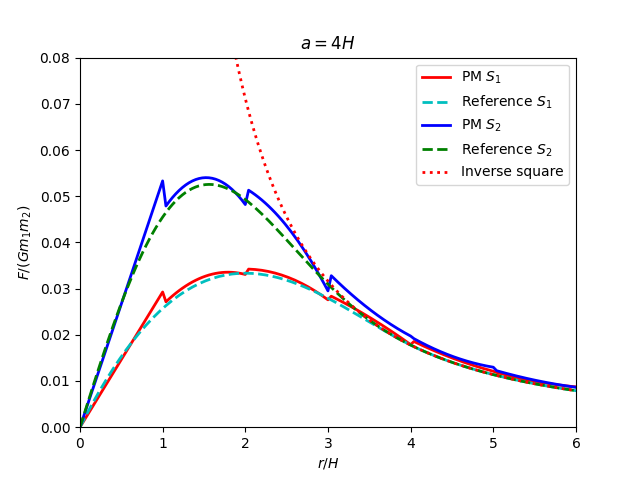
\includegraphics[width=\textwidth]{img/p3m/s1-vs-s2.png}
        \caption{Approximate vs. reference force.}
        \label{fig:reference-force-approx-sub}
    \end{subfigure}
    \hfill
    \begin{subfigure}[b]{0.48\textwidth}
        \centering
        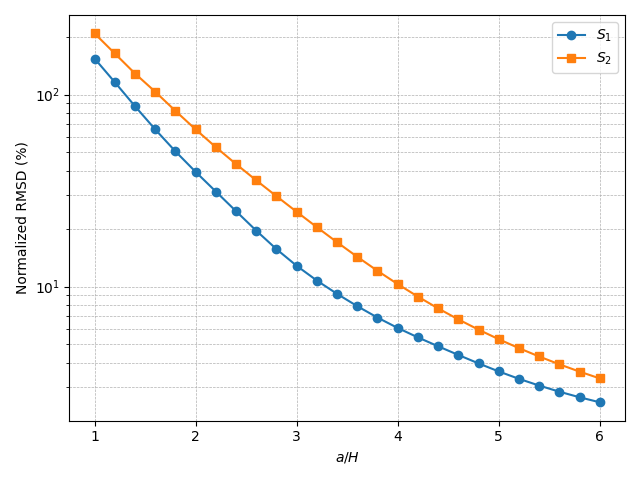
\includegraphics[width=\textwidth]{img/p3m/s1-vs-s2-nrmsd.png}
        \caption{Mean-normalized RMSD error}
        \label{fig:reference-force-error-sub}
    \end{subfigure}
    \caption{Comparison of PM approximation using $S_1$ and $S_2$ shape functions.
        The mesh approximation to the reference force was computed using the PM method with a TSC assignment scheme, two-point finite difference, and Green's function optimal for each shape.
    }
    \label{fig:reference-force-combined}
\end{figure}

The \PThreeM{} method offers a high degree of flexibility in terms of specifying the ``building blocks'' of the Green's function in \autoref{eq:optimal-greens-func}.
For example, we can be interested in learning how the choice of the assignment scheme influences the shape of the PM-approximated reference force.
The result of a test which addresses this issue is shown in \autoref{fig:reference-force-err-schemes-combined}.
\begin{figure}[htp]
    \centering
    \begin{subfigure}[b]{0.48\textwidth}
        \centering
        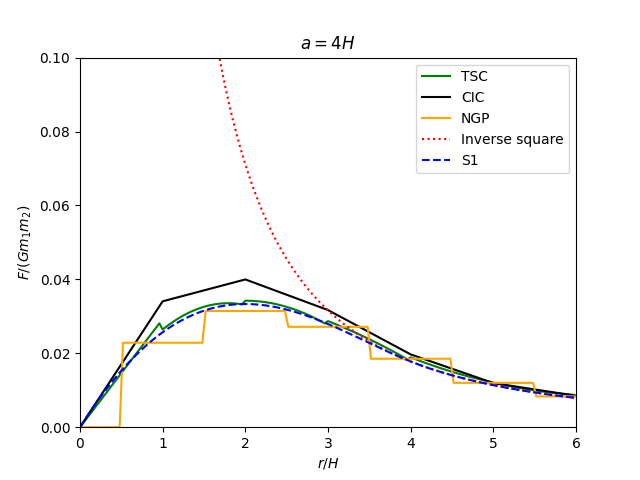
\includegraphics[width=\textwidth]{img/field_different_ass.png}
        \caption{Approximate vs. reference force.}
        \label{fig:reference-force-approx-different-schemes-sub}
    \end{subfigure}
    \hfill
    \begin{subfigure}[b]{0.48\textwidth}
        \centering
        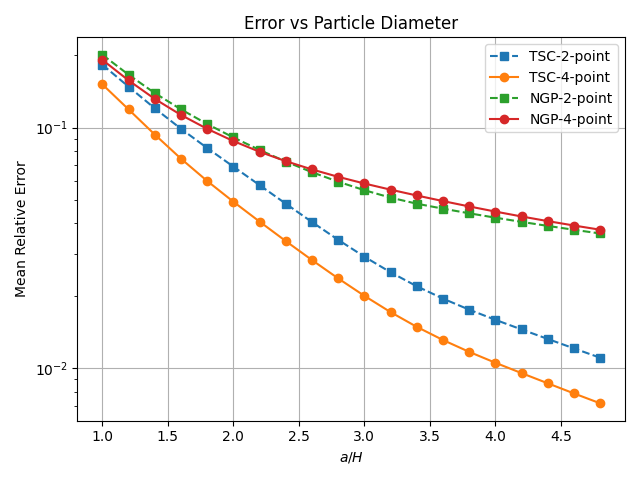
\includegraphics[width=\textwidth]{img/no-cic.png}
        \caption{Mean relative error.}
        \label{fig:reference-force-error-different-schemes-sub}
    \end{subfigure}
    \caption{Comparison of PM approximation using different assignment and interpolation functions.
    In the test we set $N=10{,}000$ and used $64\times 64\times 32$ grid.
    }
    \label{fig:reference-force-err-schemes-combined}
\end{figure}
\autoref{fig:reference-force-approx-different-schemes-sub} shows that the general characteristic of the field strength approximated by the PM method is similar to what we have already seen in \autoref{fig:pm-mass-assignment-field-strength}.
Namely, the NGP schemes yields an unnatural, jagged shape.
The shape produced using the CIC shape matches the $S_1$ reference force more closely, although it overestimates the field strength values close to the source.
The most accurate approximation is obtained using the TSC scheme (this is the same shape we have already seen in \autoref{fig:reference-force-approx-sub}).

The situation portrayed in \autoref{fig:reference-force-approx-different-schemes-sub} gives insight into a field due to a single particle.
In a typical situation, we are interested in simulating many thousands of particles and thus the averaged approximation error becomes of interest.
Just as in the case of the PM method, the global error was measured in terms of mean relative error given by \autoref{eq:force-avg-relative-err}.
This time, the error was plotted as a function of the particle diameter for TSC and NGP schemes both in two variants: using second-order and fourth-order Laplacian approximation.
The result of this test is shown in \autoref{fig:reference-force-error-different-schemes-sub}.
The figure illustrates that the error decays rapidly with increasing particle diameter when the TSC scheme is used.
It is worth noting that the fourth-order accurate finite difference yields significant improvement in accuracy for the TSC scheme-based P3M method, allowing the error to drop below $1\%$ mark for $a \approx 4H$.


To measure the quality of PM-approximation of a given reference force, we used mean-normalized RMSD error, i.e. we calculated
\begin{equation*}
    \frac{\sqrt{\frac{1}{n} \sum_{i=1}^{n} (F^\text{PM}(r_i) - R(r_i))^2}}{\frac{1}{n} \sum_{i=1}^{n} R(r_i)}
\end{equation*}
in a system with a single unit mass located on the $x$-axis.
The forces $F^\text{PM}(r_i)$ were measured along the $x$-axis in equal-length intervals and the test was run for increasing values of particle diameter $a$.
The result of the test is shown in \autoref{fig:reference-force-combined}\subref{fig:reference-force-error-sub}.
Clearly, the approximation error becomes smaller for increasing values of $a$.
Since $r_e$ is proportional to $a$, this implies that there is a tradeoff between accuracy and the execution time.
Increasing $a$ means that $r_e$ should increase as well which forces more particles into short-range correction regions.
If the system under consideration has uniform density, we note that for any given particle, the short-range correction is concerned with $\sim r_e^3$ particles in its vicinity which translates into $\sim r_e^3$ operations.
The relation between cutoff radius size $r_e$ and execution time is shown in \autoref{fig:p3m-time-vs-radius}.
\begin{figure}[htp]
    \centering
    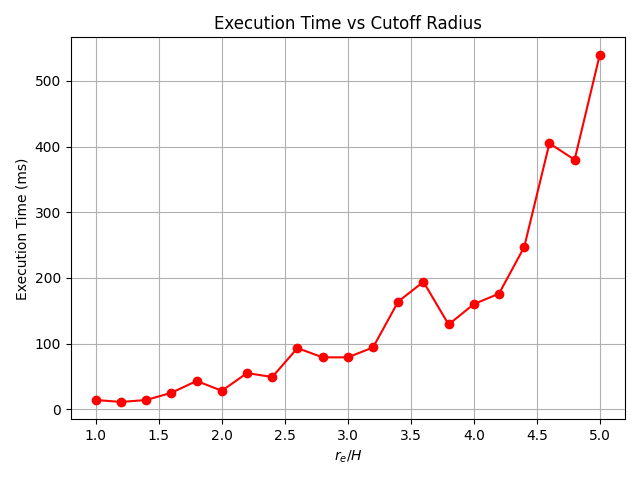
\includegraphics[scale=0.5]{img/time-vs-radius.png}
    \caption{Execution time for different setting of cutoff radius $r_e$ in the \PThreeM{} method (single step, $N=10{,}000$).
    The times shown in the graph do not include tabulating the Green's function and the PM step.}
    \label{fig:p3m-time-vs-radius}
\end{figure}
As we can see, the execution time very strongly depends on $r_e$ and this explains why choosing $r_e$ slightly even slightly less than $a$ can lead to significant improvements in performance.
Another conclusion that can be drawn from \autoref{fig:reference-force-error-sub} is that the \( S_2 \)-based approximation exhibits higher mean-normalized RMSD error compared to \( S_1 \).
However, as we remarked previously, it allows for choosing $r_e \lesssim a$ without significant loss of accuracy.
Therefore, the choice between \( S_1 \) and \( S_2 \) shapes involves a trade-off between accuracy near the source and overall error, making the optimal choice context-dependent.


\subsection{Identifying close pairs of particles}
In the \PThreeM{} method, in addition to the mesh used in the PM algorithm (the ``potential mesh''), a second mesh (the \textit{chaining mesh}) is used.
The chaining mesh is sparser than the potential mesh.
Its sole purpose is to partition the space into cells so that particles ``close'' to the ones in a given cell can be found efficiently.
In this context, two particles are considered to lie close to one another if their separation is less than the cutoff radius.

The number of chaining mesh cells in a single dimension is given by $M_i = \lfloor L_i / r_e \rfloor$, where $L_i$ is the side length of the computational box ($i=1,2,3$).
This implies that the side length of a chaining mesh cell is $\text{HC}_i = L_i / M_i \geq r_e$.
Thus, for every particle $i$ in a given cell $\mathbf{p}$, it is sufficient to search through the immediate neighborhood of $\mathbf{p}$ to find all the particles within the cutoff radius from $i$.

In our program, the chaining mesh is implemented as a \textit{head-of-chain} (HOC) array, depicted in \autoref{fig:hoc}.
\begin{figure}[htp]
    \centering
    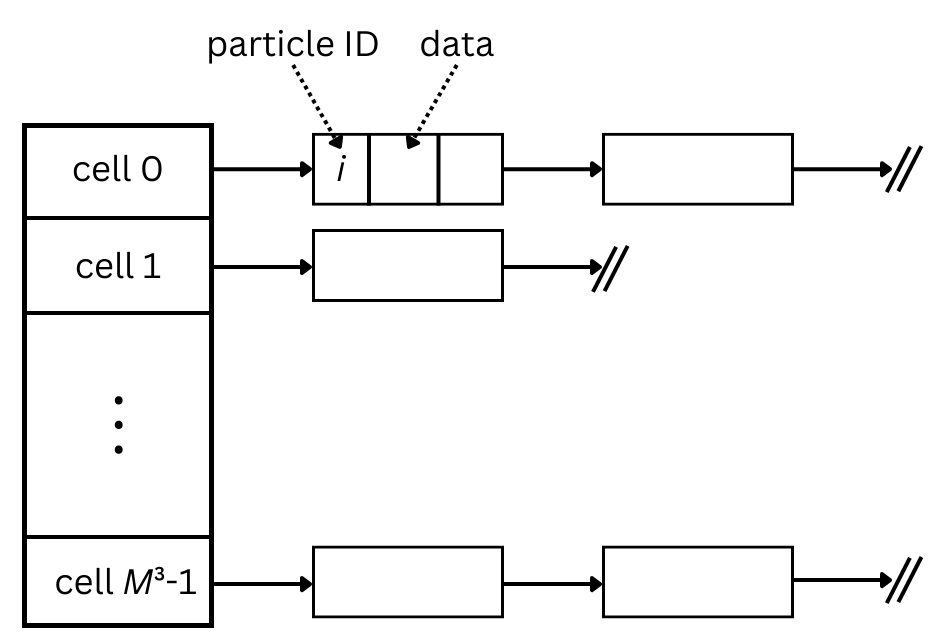
\includegraphics[scale=0.25]{img/hoc.png}
    \caption{Head-of-chain data structure used for mapping particles to their parent cells in the chaining mesh.
        Here $M_1=M_2=M_3 = M$.}
    \label{fig:hoc}
\end{figure}
The basic version of the HOC array is very cheap to build.
Given a particle at point $\mathbf{x} = (x, y, z)$, we can determine in which chaining mesh cell $\mathbf{c}$ it lies by simply performing integer division on each of its coordinates, i.e. $\mathbf{c} = (x / \text{HC}_1, y / \text{HC}_2, z / \text{HC}_3)$.
Then, to get a HOC table index $i$ corresponding to $\mathbf{c}$, standard index flattening is used.
Subsequently, a new linked-list node is allocated and inserted at the beginning of the list HOC[$i$].
Clearly, the whole process is linear in the number of particles and the array can be constructed anew at each time step without degrading performance.
In our implementation, additional savings are made by preallocating a memory pool large enough to store $N$ nodes of the linked lists and reusing it for the HOC array initialization.

A potential optimization discussed in \cite{Hockney1988} involves sorting each linked list by a selected particle coordinate, such as the $y$-coordinate.
This ordering enables early termination of the direct summation loop when the condition $y_i - y_j > r_e$ is met, effectively reducing unnecessary pairwise computations as particle $i$ "sweeps through" a cell containing particles $j$.
Our experiments indicate that constructing the linked lists in sorted order is substantially more expensive than the unsorted variant.
This is to be expected; in the worst-case scenario where all particles are in a single chaining-mesh cell, and are inserted into the list in decreasing order of $y$ coordinates, the complexity is $O(N^2)$.
For a system of 50{,}000 particles, incorporating $y$-sorting increased the HOC (head-of-chain) construction time from approximately 180 milliseconds to over 13{,}000 milliseconds, a 70-fold slowdown.
Despite this added cost, we observed no significant performance improvement in the short-range correction phase of the computation.

\subsection{Short-range correction}
The short-range correction, which takes place immediately after the mesh forces are found using the PM method, is at the heart of the \PThreeM{} algorithm.
Since it scales with a square of the number of particles in each neighborhood, further optimizations are highly desirable.

By Newton's 3rd law, $\mathbf{f}^\text{SR}_{ji} = -\mathbf{f}^\text{SR}_{ij}$, which allows us to do the calculation of the short-range inter-particle force for any pair $(i, j)$ of particles only once, leading to the reduction of the total running time by half.
Informally, the particle $i$ updates its total short-range force $\mathbf{F}^\text{SR}_i$ as well as the total short-range force $\mathbf{F}^\text{SR}_j$ of its neighbor $j$.
To avoid double-counting, the particle $i$ residing in cell $\mathbf{q}$ has to look for its neighbors in a subset $\mathcal{N}$ of the immediate neighborhood of $\mathbf{q}$.
More specifically, define
\begin{equation}\label{eq:n-set}
    \mathcal{N}(\mathbf{q} = (q_1, q_2, q_3)) = \{(q_1+t, q_2-1,q_3+s), (q_1+s, q_2, q_3-1), (q_1-1,q_2,q_3) \;|\; s,t = -1,0,1 \}.
\end{equation}
Thus $|\mathcal{N}| = 13$, which is half of the size of the immediate neighborhood.
The set $\mathcal{N}$ given in \autoref{eq:n-set} is not easily to illustrate.
Since for the purposes of the later discussion, it is beneficial to have a clear picture in mind, we depict its two-dimensional analog in \autoref{fig:n-set-2d}.
\begin{figure}[htp]
    \centering
    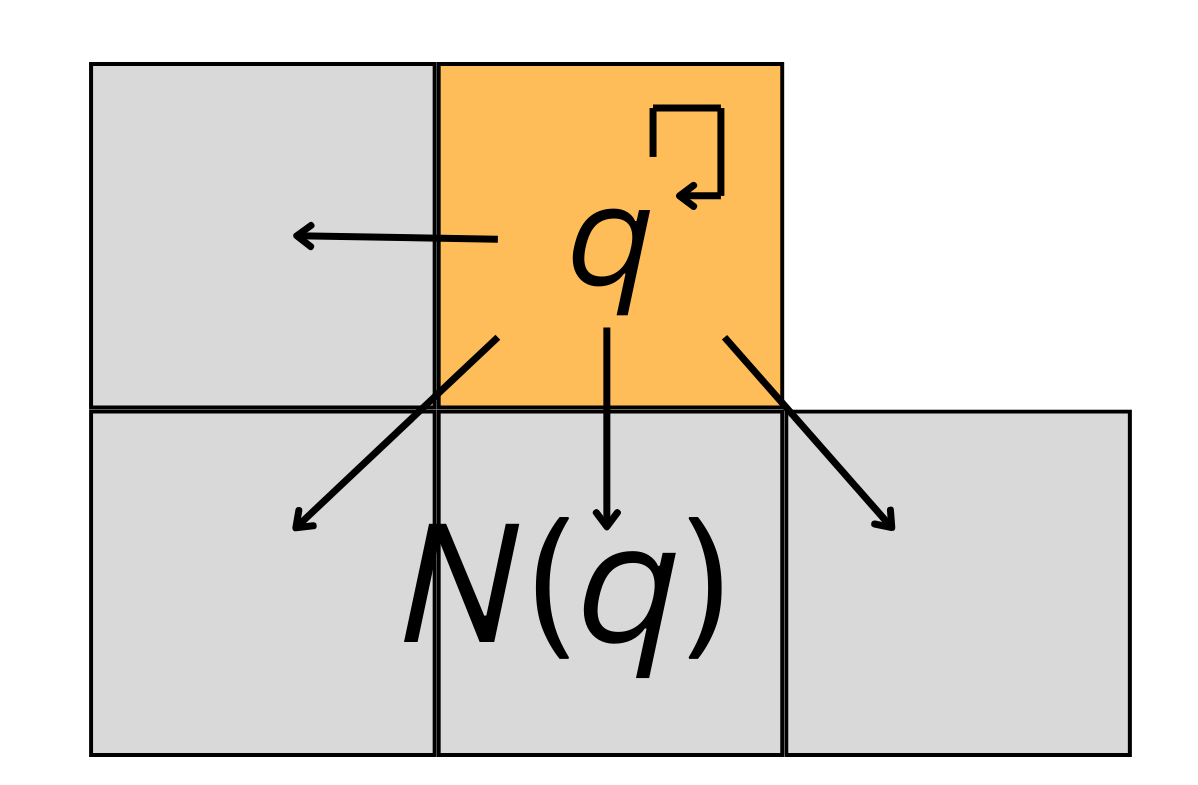
\includegraphics[scale=0.12]{img/q-neighborhood.png}
    \caption{Set $\mathcal{N}$ in two dimensions.}
    \label{fig:n-set-2d}
\end{figure}

The short-range correction part of the \PThreeM{} method is shown in \autoref{alg:short-range-correction}.
\begin{algorithm}
    \caption{Short-range correction}\label{alg:short-range-correction}
    \begin{algorithmic}[1]
        \ForAll {chaining cell $\mathbf{q}$}
        \ForAll {$\mathbf{q}_n \in \mathcal{N}(\mathbf{q}) \cup \{\mathbf{q}\}$}
        \ForAll {$i \in \text{HOC}(\mathbf{q})$}
        \ForAll {$j \in \text{HOC}(\mathbf{q}_n)$}
        \If {$|y_i - y_j| > r_e$}
        \Break
        \EndIf
        \State \Call{UpdateShortRange}{$i$, $j$, $\mathbf{q}$, $\mathbf{q}_n$}
        \EndFor
        \EndFor
        \EndFor
        \EndFor
    \end{algorithmic}
\end{algorithm}
For each chaining mesh cell $\mathbf{q}$, we compute the pair-wise interactions between the particles in $\mathbf{q}$ and the particles in the chaining mesh cells $\mathbf{q}_n$ from the reduced neighborhood $\mathcal{N}(\mathbf{q})$ \textit{plus} $\mathbf{q}$.
The inclusion of $\mathbf{q}$ allows us to take into account forces between particles within $\mathbf{q}$.

The \textsc{UpdateShortRange} procedure is defined in \autoref{alg:update-short-range-forces}.
\begin{algorithm}
    \caption{Updating short-range forces}\label{alg:update-short-range-forces}
    \begin{algorithmic}[1]
        \Procedure{UpdateShortRange}{$i$, $j$, $\mathbf{q}$, $\mathbf{q}_n$}
        \If {$i = j$}
        \Return
        \EndIf
        \State $\mathbf{r}_{ij} \gets \mathbf{r}_i - \mathbf{r}_j$
        \If {$|\mathbf{r}_{ij}|^2 > r_e^2$}
        \Return
        \EndIf
        \State $r_{ij} \gets |\mathbf{r}_{ij}|$
        \State $\mathbf{\hat{r}}_{ij} \gets \mathbf{r}_{ij} / r_{ij}$
        \State $\mathbf{R}_{ij} \gets -m_i m_j R(r_{ij}) \mathbf{\hat{r}}_{ij}$
        \State $\mathbf{f}^\text{tot} \gets -G m_i m_j / r_{ij}^2 \mathbf{\hat{r}}_{ij}$
        \State $\mathbf{f}^\text{SR}_{ij} \gets \mathbf{f}^\text{tot} - \mathbf{R}_{ij}$
        \State $\mathbf{f}^\text{SR}_{ji} \gets -\mathbf{f}^\text{SR}_{ij}$
        \State $\mathbf{F}^\text{SR}_i \gets \mathbf{F}^\text{SR}_i + \mathbf{f}^\text{SR}_{ij}$
        \If {$\mathbf{q}_n \neq \mathbf{q}$} \Comment{Avoid double-counting in the parent cell}
        \State $\mathbf{F}^\text{SR}_j \gets \mathbf{F}^\text{SR}_j + \mathbf{f}^\text{SR}_{ji}$
        \EndIf
        \EndProcedure
    \end{algorithmic}
\end{algorithm}
In line 2, we exclude self-forces.
The check in line 4 assures that the correction happens only for particles with separation less than the cutoff radius $r_e$.
The pair-wise short-range force is calculated in lines 5--10, with the calculation in line 10 exploiting the Newton's third law, as described previously.
The accumulation of total short-range force for a given particle takes place in line 11.
The short-range force is also added to the total short-range force of the other particle in the pair (particle $j$) but only if $\mathbf{q}_n \neq \mathbf{q}$.
This stipulation is crucial, as otherwise we would be double counting the forces between particles within $\mathbf{q}$.

As suggested in \cite{Hockney1988}, the computational burden of operations in lines 5--8 in \autoref{alg:update-short-range-forces} can be greatly reduced by storing the values of $f^\text{SR}(r) / r = (f^\text{tot}(r) - R(r)) / r$ in a lookup table $T$ at uniform intervals $\Delta^2$ of $[0, r_e^2]$ and interpolating them later.
The schematic depiction of the interpolation is shown in \autoref{fig:sr-force-val-interpolation}.
\begin{figure}[htp]
    \centering
    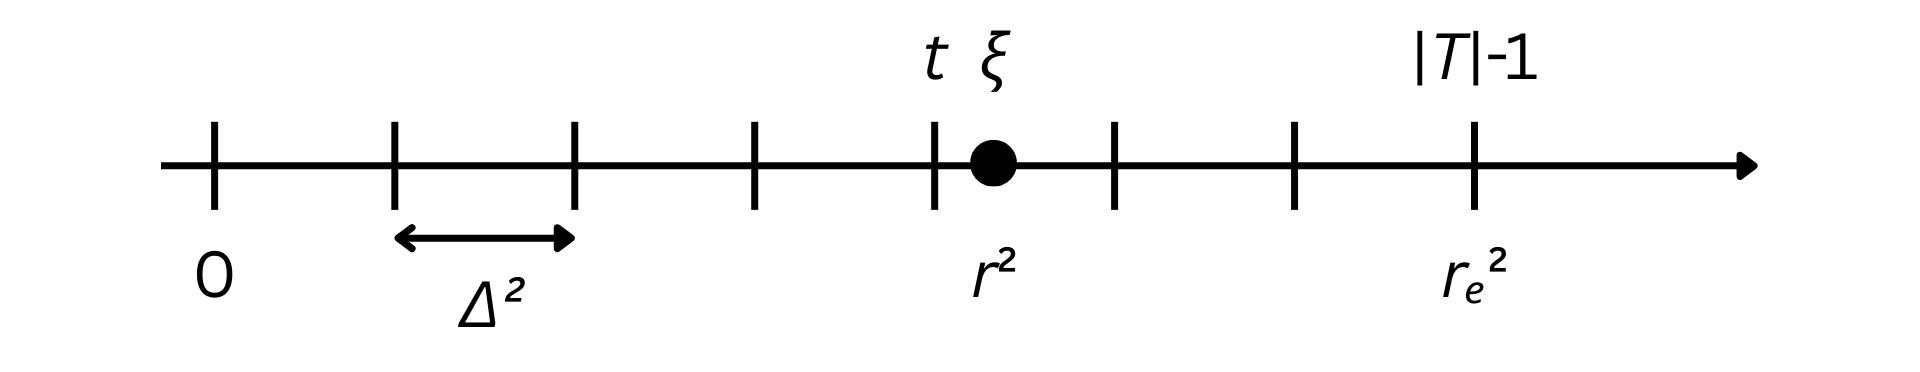
\includegraphics[scale=0.2]{img/interpolation.png}
    \caption{Interpolation of short-range force values.}
    \label{fig:sr-force-val-interpolation}
\end{figure}
If we define $\xi = r^2 / \Delta^2$ and $t=\lfloor \xi \rfloor$, then
\begin{equation*}
    \frac{f^\text{SR}(r)}{r} \approx T[t]\left(1 - (\xi - t)\right) + T[t+1](\xi - t)
    = T[t] + (\xi - t) (T[t+1] - T[t]).
\end{equation*}
The value $\mathbf{f}^\text{SR}_{ij}$ can then be obtained by multiplying the interpolated quantity $f^\text{SR}(r_{ij})/r_{ij}$ by $G m_i m_j \mathbf{r}_{ij}$, eliminating the use of the square root operations and reducing the total number of floating-point operations to just four.

In our implementation, the procedure outlined in\autoref{alg:short-range-correction} is parallelized by splitting the work done in the outmost loop between some number of threads.
In doing so, extra care has to be taken to avoid data races.
A thread $t$ that is currently processing cell $\mathbf{p}$ and its neighbors (we say that $t$ is \textit{assigned} to $\mathbf{p}$) may ``clash'' with a different thread assigned to a nearby cell $\mathbf{q}$ (because possibly $\mathbf{p} \in \mathcal{N}(\mathbf{q})$).
However, by the construction of the set $\mathcal{N}$, it is possible to split the short-range force into 14 parts, each of which is accessed by only one thread.
For example, consider a particle $i$ in cell $\mathbf{p} = (p_1, p_2, p_3)$ (in other words, $\mathbf{p}$ is the parent cell of $i$).
If thread $t$ is currently assigned to this cell, $t$ will update the part of $\mathbf{F}^\text{SR}_i$ corresponding to updates of $i$ coming from within the same cell as the parent cell of $i$.
Possibly at the same time, thread $t'$ assigned to cell $\mathbf{q} = (p_1+1, p_2, p_3)$ will update a different part of $\mathbf{F}^\text{SR}_i$, i.e. the part corresponding to updates of $i$ coming from the cell ``to the right'' of the parent cell of $i$.
Since only one thread is responsible for updates to particle $i$ coming ``from the right,'' (or any other ``direction'') no data races can occur.
This approach presents two major drawbacks.
First, it significantly increases memory usage, requiring storage for an additional $13N$ three-dimensional vectors.
Second, it offers no guarantee of uniform workload distribution across threads.
This imbalance, combined with the substantial variation in operations performed by individual threads, leads to severe thread divergence, rendering the parallelization scheme unsuitable for GPU execution.

\subsection{Force approximation error and performance}
The ``local picture'' of the errors of force approximation in the \PThreeM{} method has already been outlined in \autoref{fig:reference-force-combined}.
Now we turn to investigate how the choice of the particle shape ($S_1$ or $S_2$) and the size of the particle diameter influences the global force approximation error.
The error is defined exactly the same as in the case of the PM method, i.e. we use \autoref{eq:force-avg-relative-err}.

In our test, the grid covering the computational region had dimensions of $64\times 64\times 32$ and $N=10{,}000$ particles were used.
The result of the test is shown in \autoref{fig:p3m-global-err}.
\begin{figure}[htp]
    \centering
    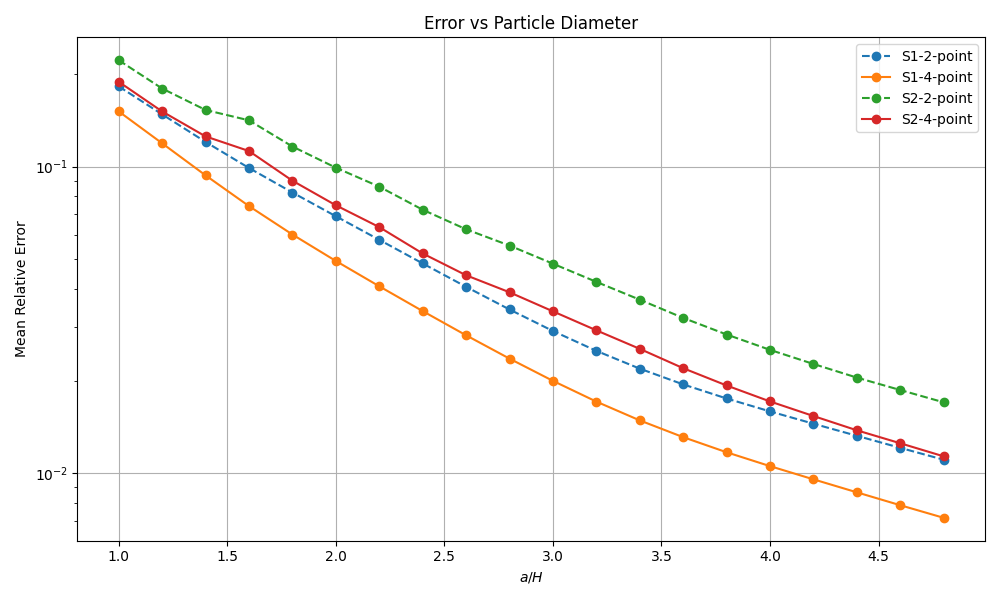
\includegraphics[scale=0.5]{img/err_vs_part_diam_p3m.png}
    \caption{Mean relative error in P3M approximation.}
    \label{fig:p3m-global-err}
\end{figure}
The figure clearly illustrates that the error drops with increasing the size of the particle diameter $a$.
This is an expected result, since with increasing $a$, the P3M method calculates more interparticle forces through exact direct summation.
Moreover, as we could see in \autoref{fig:reference-force-error-sub}, the PM approximation to the reference force gets better with increasing particle diameter.
These two effects combined are responsible for the reduction of the global error.

For both the $S_1$ and $S_2$ shapes, the error was minimized when the fourth-order finite difference was used for gradient calculation, as one could obviously expect.
The test indicated superiority of the $S_1$ shape, with the difference between the two becoming more significant for bigger relative values of $a$.